\section{Utente non autenticato}
Come utente non autenticato, hai accesso a una serie di funzionalità di base che 
ti permettono di esplorare EasyMeal e di accedere o registrarti.

\subsection{Header}

\begin{figure}[htbp]
    \centering
	
\includegraphics[width=0.8\textwidth]{PB/manuale-utente/header-non-autenticato.png}
    \caption{Barra di Navigazione per l'utente non autenticato}
\end{figure}

La barra di navigazione in alto ti permette di accedere facilmente alle varie 
sezioni della piattaforma. 
Puoi tornare alla schermata principale cliccando sul logo EasyMeal o sul nome 
EasyMeal entrambi posti in alto a sinistra. Allo stesso modo si può cliccare su
\texttt{Esplora} per effettuare la medesima operazione. Infine, si può cliccare
su \texttt{Login} per accedere alla schermata di login e su 
\texttt{Registrati} per accedere alla schermata di registrazione.

\subsection{Footer}

\begin{figure}[htbp]
    \centering
	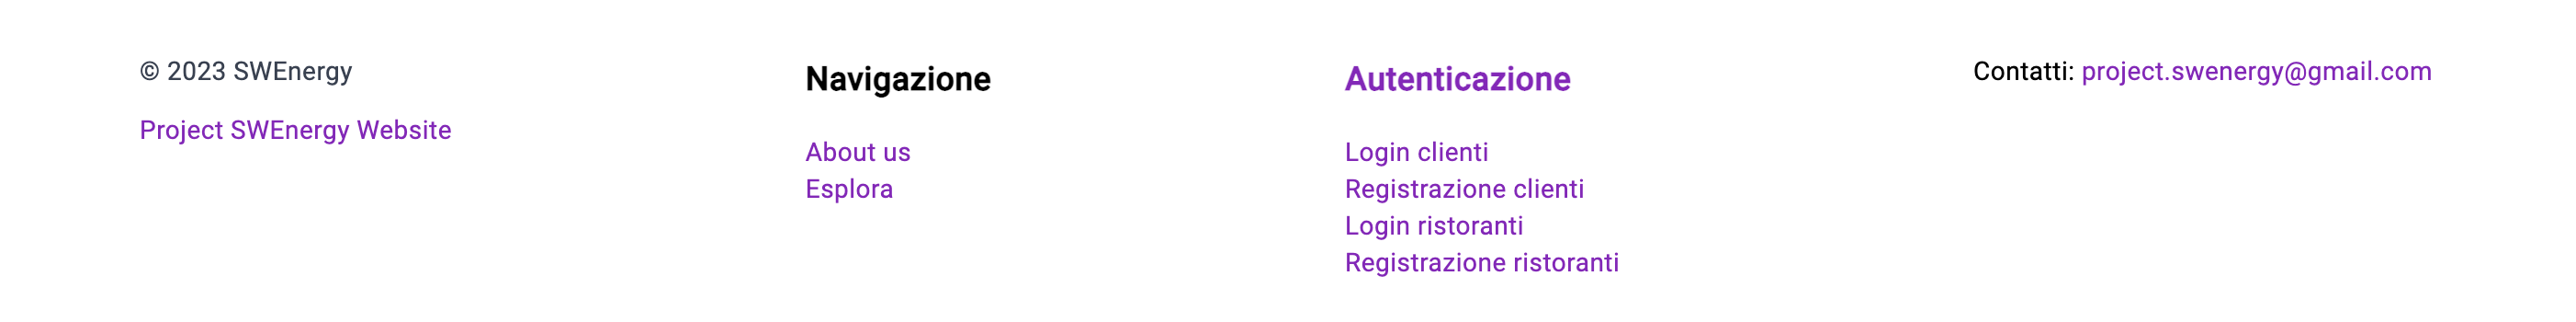
\includegraphics[width=0.8\textwidth]{PB/manuale-utente/footer.png}
    \caption{Footer}
\end{figure}

Il footer si trova in fondo ad ogni pagina. In viola sono evidenziati i link
cliccabili che ti permettono di accedere alle sezioni di EasyMeal. In
particolare, da sinistra verso destra, dall'alto verso il basso si ha:
\begin{itemize}
	\item \textbf{\texttt{Project SWEnergy Website}}: questo collegamento permette di
		accedere al sito web del gruppo SWEnergy, che ha sviluppato EasyMeal.
		In particolare, il sito contiene informazioni sul gruppo e i documenti
		del progetto EasyMeal;

	\item \textbf{Navigazione}: sotto questa voce sono presenti i link "About
		us" e "Esplora". Il primo link è collegato ad una pagina che introduce
		il progetto EasyMeal. Il secondo riporta alla pagina di esplorazione dei
		ristoranti;

	\item \textbf{\texttt{Autenticazione}}: questa voce rimanda ad una pagina di
		selezione della tipologia di login e di registrazione. In particolare,
		si tratta di una pagina dedicata alle quattro voci sotto di essa. Sotto
		questa voce sono presenti i link \texttt{Login clienti}, 
		\texttt{Registrazione clienti}, \texttt{Login ristoratori} e 
		\texttt{Registrazione ristoratori}. Questi
		link permettono di accedere alle pagine di login e registrazione per
		clienti e ristoratori;

	\item \textbf{Contatti}: viene mostrata la mail di contatto del gruppo
		SWEnergy, per permettere agli utenti di contattare il gruppo per
		eventuali problemi o domande;
\end{itemize}


\subsection{Home Page}

\begin{figure}[htbp]
    \centering
	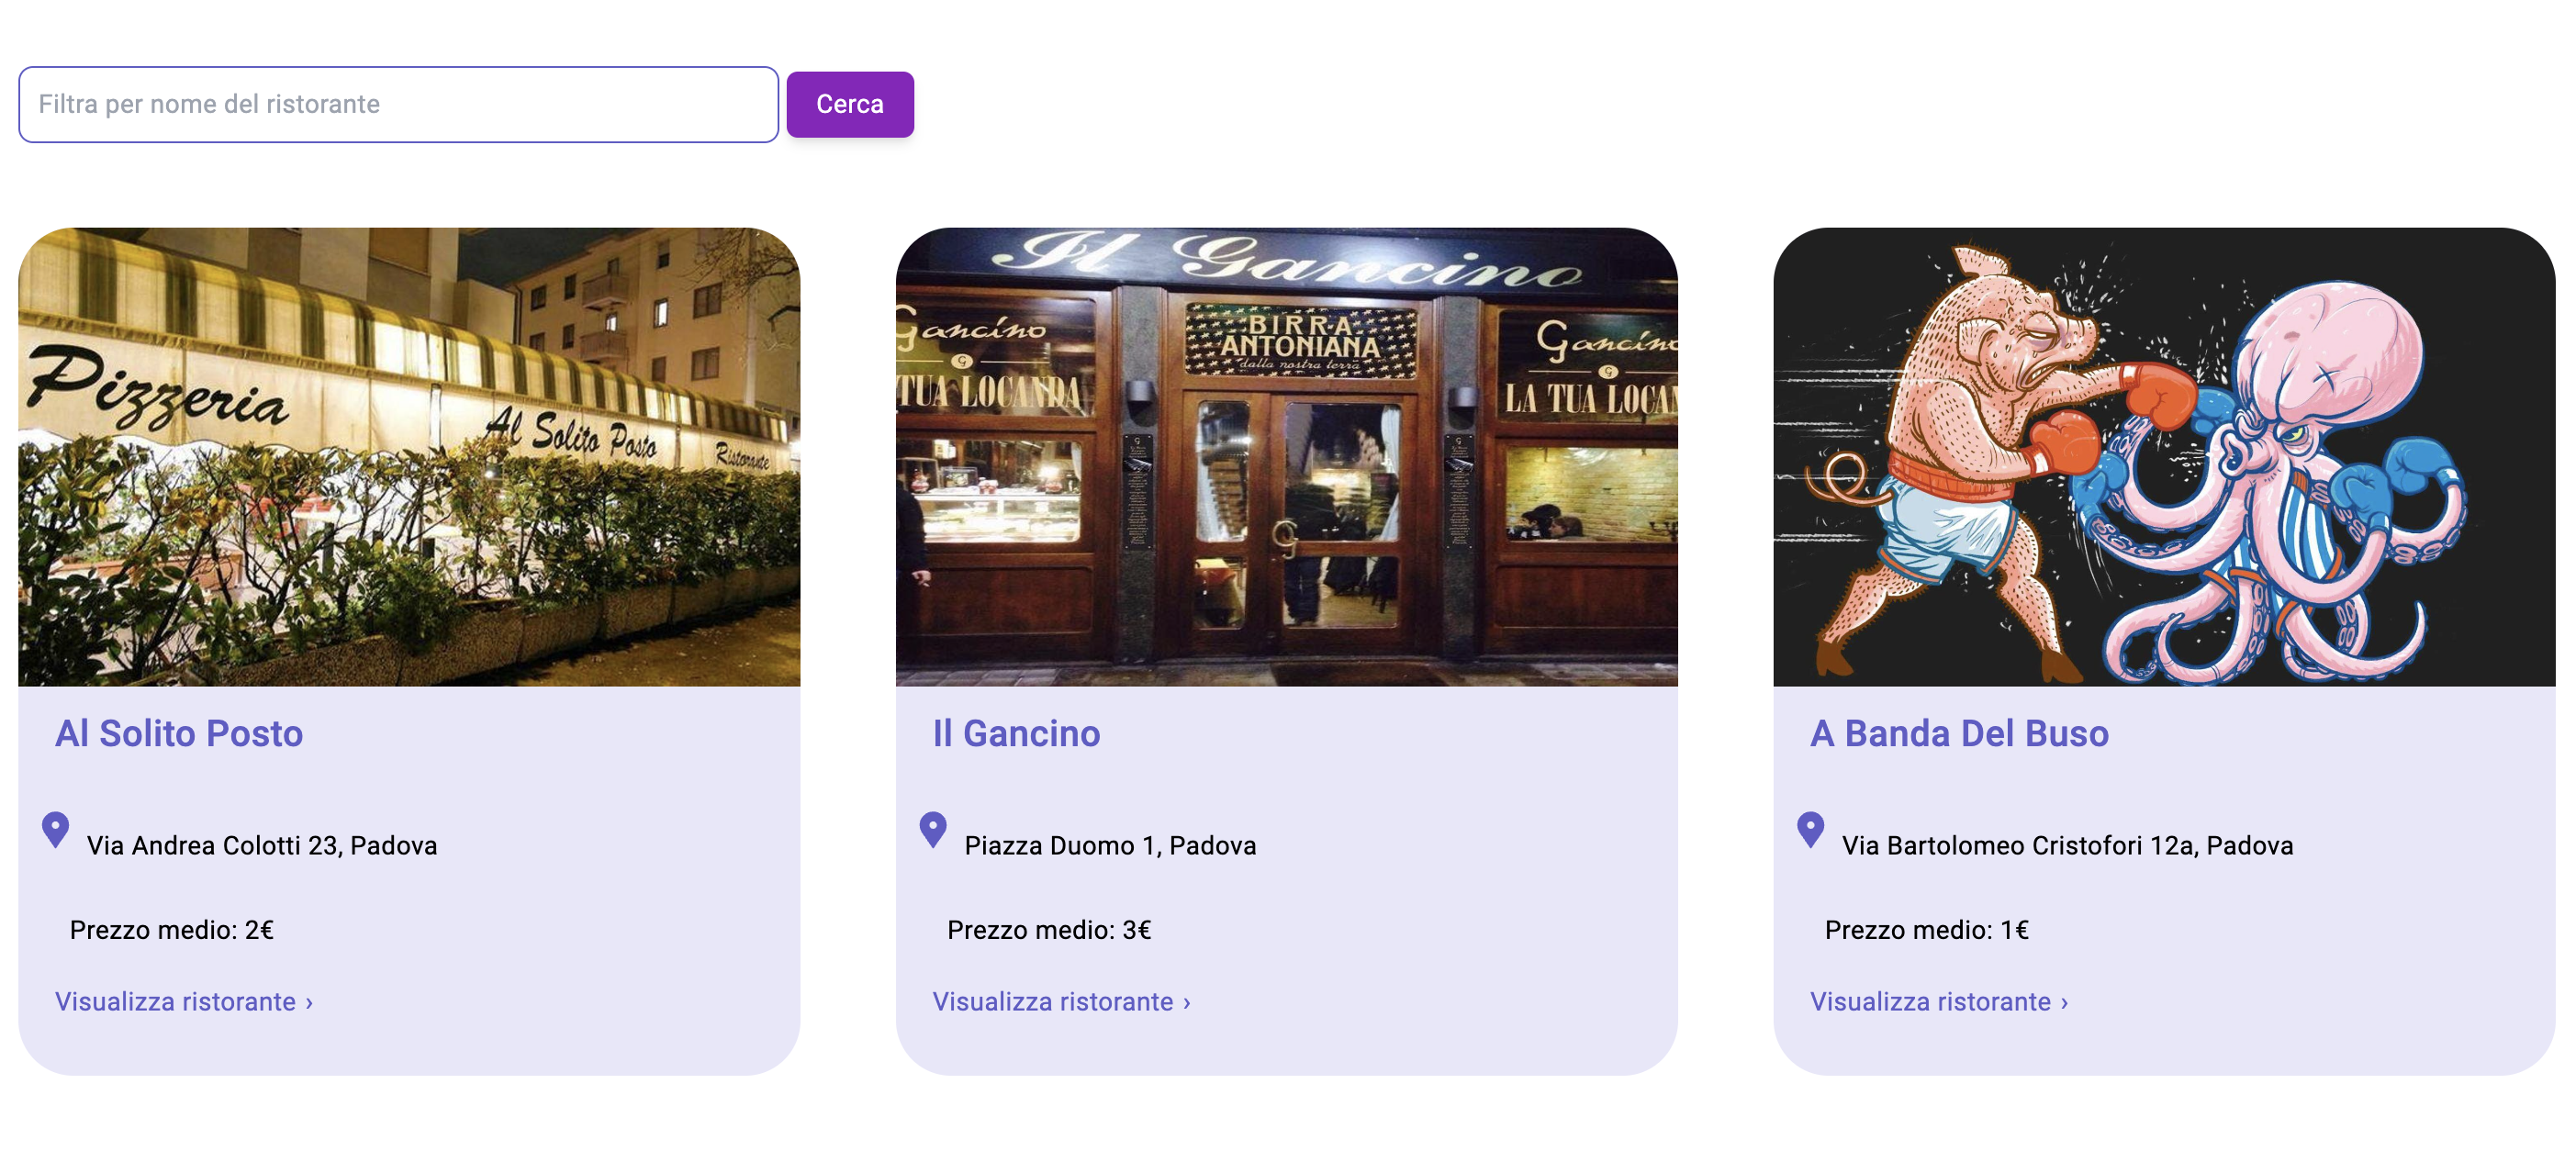
\includegraphics[width=0.8\textwidth]{PB/manuale-utente/home-non-autenticato.png}
    \caption{Home Page per l'utente non autenticato}
\end{figure}

La Home Page è il punto di ingresso principale per gli utenti non autenticati. 
Sono mostrati i ristorati presenti su EasyMeal e le loro informazioni
principali. In cima all'elenco è presente un campo di ricerca per trovare
rapidamente un ristorante conoscendone il nome. Infine, sotto a ciascun
ristorante è presente un riferimento cliccabile \texttt{Visualizza ristorante >}
che permette di visualizzare in dettaglio le informazioni del ristorante.

\subsection{Visualizza in dettaglio un ristorante}

\begin{figure}[htbp]
    \centering
	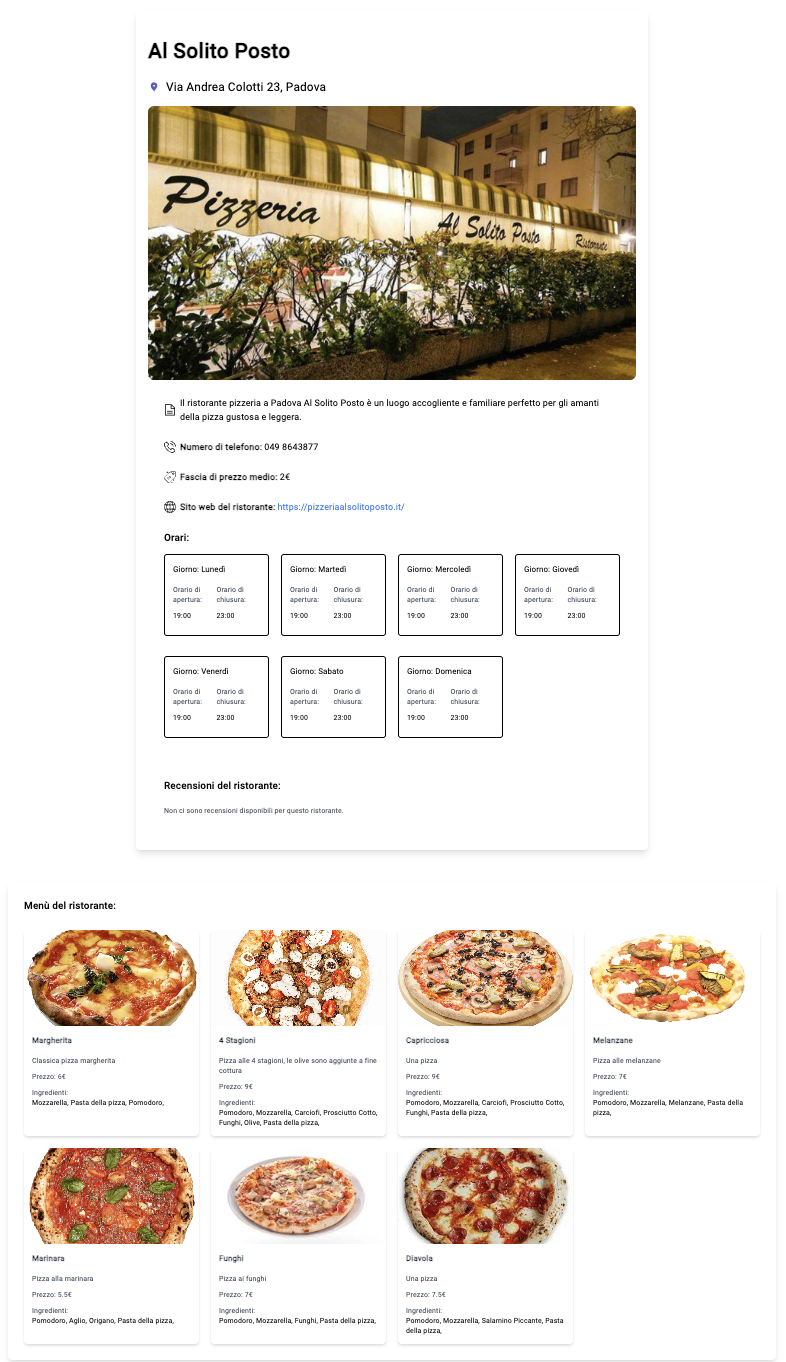
\includegraphics[width=0.8\textwidth]{PB/manuale-utente/dettagli-ristorante-non-autenticato.png}
    \caption{Pagina di visualizzazione in dettaglio di un ristorante per l'utente non autenticato}
\end{figure}

Nella seguente pagina sarà possibile visualizzare tutte le informazioni relative 
al ristorante e inoltre sarà possibile visualizzare il menu del ristorante, con 
i relativi piatti e prezzi e inoltre visualizzare le recensioni del ristorante.
Infine, copiando il link del ristorante è possibile condividerlo con chiunque,
infatti questo link è univoco per ogni ristorante e permette di accedere 
direttamente alla pagina di visualizzazione in dettaglio del ristorante.

\subsection{Login cliente}

\begin{figure}[htbp]
    \centering
	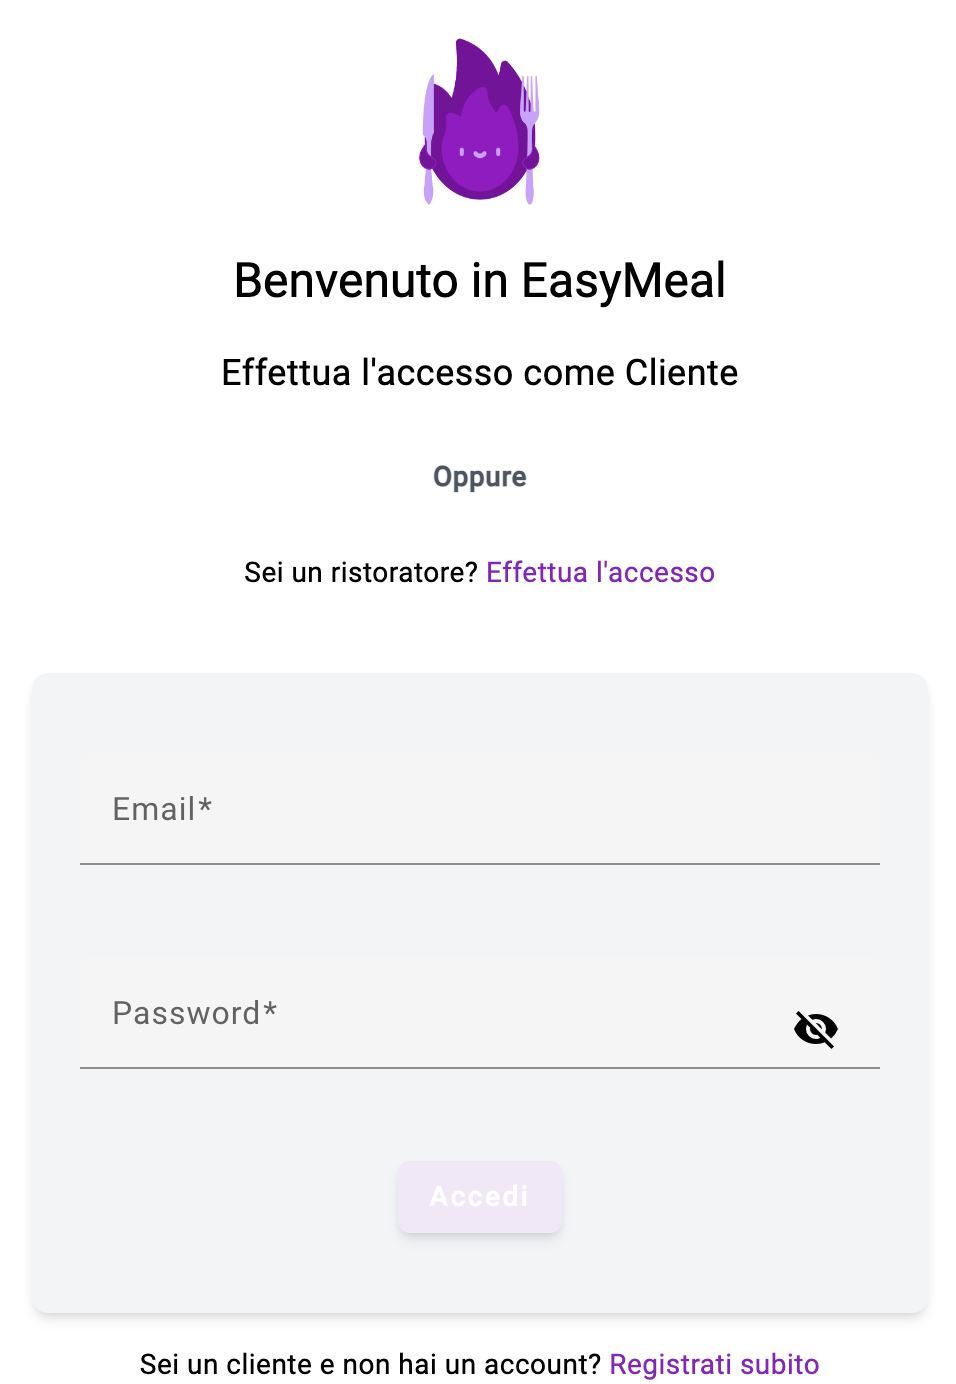
\includegraphics[width=0.3\textwidth]{PB/manuale-utente/login-cliente.png}
    \caption{Pagina di login lato utente cliente}
\end{figure}

In questa pagina è presente un form di login per permettere agli utenti di
accedere alla propria area persona. In particolare, è necessario inserire
l'indirizzo email e la password corrispondente. Una volta inseriti i dati è
possible cliccare sul pulsante \texttt{Accedi} per procedere con 
l'autenticazione. Se l'autenticazione avviene con successo, verrà mostrata una
notifica in basso a destra indicante "Utente autenticato". Se ci sono errori
durante l'autenticazione verrà mostrato un messaggio di errore appropriato.\\
In cima al form, è presente un link cliccabile "Sei un ristoratore?
\texttt{Effettua l'accesso}" che permette di accedere alla pagina di login per
i ristoratori. In fondo al form, è presente un link cliccabile "Sei un cliente e 
non hai un account? \texttt{Registrati}" che permette di accedere alla pagina di 
registrazione per gli utenti clienti.

\subsection{Login ristoratore}

La pagina di login del ristoratore è analoga a quella del cliente. In
particolare è possibile accedere alla pagina di login per i ristoratori 
cliccando sul link "Sei un ristoratore? \texttt{Effettua l'accesso}" presente 
nella pagina di login per i clienti, oppure cliccando sul link 
"Login ristoratori" presente nel footer di ogni pagina.

\subsection{Registrazione cliente}

\begin{figure}[htbp]
    \centering
	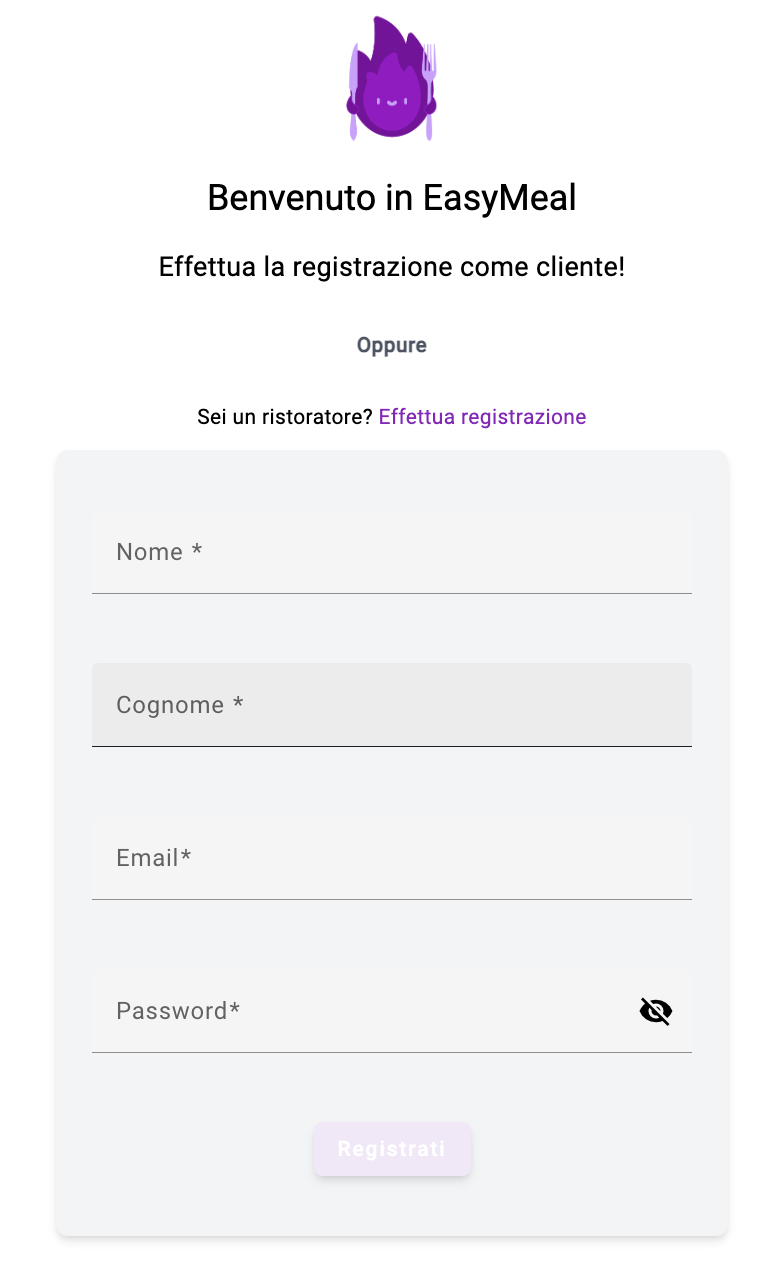
\includegraphics[width=0.3\textwidth]{PB/manuale-utente/registrazione-cliente.png}
    \caption{Pagina di registrazione lato utente cliente}
\end{figure}

Per registrarti come nuovo cliente, compila il form di registrazione con le
seguenti infomazioni:

\begin{itemize}
	\item Nome e cognome;
	\item Indirizzo email;
	\item Password;
\end{itemize}

Una volta completato il form e inviata la richiesta di registrazione, riceverai 
una notifica in basso a destra indicante 
``Utente creato con successo'' se la registrazione è avvenuta con successo.
Altrimenti, è visualizzato un messaggio di errore se ci sono problemi durante il
processo di registrazione.\\
In cima al form di registrazione, è presente un link "Sei un ristoratore?
\texttt{Effettua la registrazione}" che permette di accedere alla pagina di
registrazione per i ristoratori.

\subsection{Registrazione ristoratore}

\begin{figure}[htbp]
    \centering
	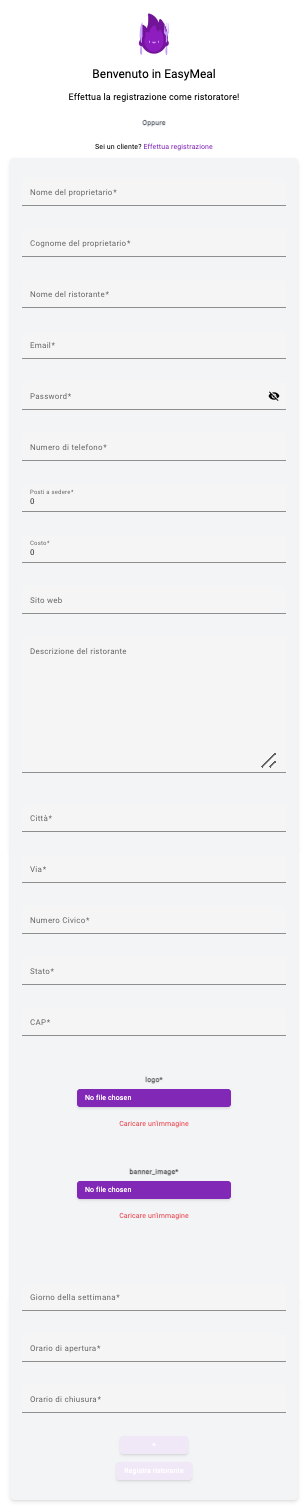
\includegraphics[width=0.3\textwidth]{PB/manuale-utente/registrazione-ristoratore.png}
    \caption{Pagina di registrazione lato utente cliente}
\end{figure}

Per registrarti come nuovo ristoratore, compila il form di registrazione con le
seguenti informazioni:
\begin{itemize}
	\item Nome e cognome del proprietario;
	\item Nome del ristorante;
	\item Indirizzo email;
	\item Password;
	\item Numero di telefono;
	\item Posti a sedere;
	\item Costo (da 0 a 3, dove 0 è il minimo e 3 il massimo);
	\item Indirizzo del sito web del ristorante (opzionale);
	\item Descrizione del ristorante (opzionale);
	\item Città;
	\item Via;
	\item Numero civico;
	\item Stato;
	\item CAP;
	\item Il logo del ristorante;
	\item Il banner del ristorante;
	\item Orari di apertura e chiusura per ciascun giorno della settimana.
\end{itemize}

Una volta completato il form e inviata la richiesta di registrazione, riceverai 
una notifica in basso a destra che indica il successo o il fallimento
dell'operazione.

In particolare, dopo aver compilato il form di inserimento di un giorno con
relativo orario di apertura e chiusura, è possibile cliccare sul pulsante
\texttt{+} per aggiungere un altro giorno. Una volta aggiunto un orario, è
possibile rimuoverlo cliccando sul pulsante \texttt{X} a destra del suddetto
orario.\\
In cima al form di registrazione, è presente un link "Sei un cliente? \texttt{Effettua la registrazione}"
